\specsection{2.2 Сформулировать определения случайной величины и функции распределения случайной
величины. Сформулировать определения дискретной и непрерывной случайной величины.
Доказать свойства плотности распределения вероятностей непрерывной случайной величины.}

\OPR Случайной величиной называют функцию $X:\Omega\rightarrow\mathbb{R}$, такую, что для $\forall x\in\mathbb{R}$ мн-во $\{\omega : X(\omega)<x\}\in \beta$ (т.е. это мн-во является событием)

\OPR Функцией распределения (вероятностей) случ. величины $X$ называется отображение $F:\mathbb{R}\rightarrow\mathbb{R}$, определённое условием $F(x) = P\{X<x\}$

\OPR Сл. вел. $X$ называется дискретной, если мн-во её значений конечно или счётно

\OPR Сл. вел. $X$ называется непрерывной, если существует ф-ия $f(x)$ такая что, ф-ия распред. случ. вел. $X$ м. б. представлена в виде $F(x)=\intl_{-\infty}^{x}f(t)dt$

Свойства ф-ии плотности распределения
\begin{enumerate}[topsep=0pt, leftmargin=20pt, noitemsep, label=\arabic*\degree]
	\item $f(x)\geq 0,~x\in\mathbb{R}$
	
	\item $P\{x_1\leq X \leq x_2\}=\intl_{x_1}^{x_2}f(x)dx$
	
	\item $\intl_{-\infty}^{+\infty}f(x)dx=1$
	
	\item Если $x_0$ точка непрер. $f(x)$, то при малых $\varDelta x~P\{x_0\leq X \leq x_0+\varDelta x\}\approx f(x_0)\varDelta x$
	
	\item Если $X$ -- непрер. сл. вел., то для любого наперёд заданного $x_0~~P(X=x_0)=0$
	
	\item [] Доказательства
	
	\setcounter{enumi}{0}
	
	\item $f(x)=F'(x)$, т.к. $F(x)$ -- неуб. ф-ия, то $F'(x)\geq 0\Rightarrow f(x)\geq 0$
	
	\item По свойству функции распределения $P\{x_1\leq X \leq x_2\}=F(x_2)-F(x_1)=|$ т.к. $F(x)$ -- первообразная для $f(x)|\stackrel{\text{ф-ла Ньютона-Лейбница}}{=}\intl_{x_1}^{x_2}f(x)dx$
	
    \item $\intl_{-\infty}^{+\infty}f(x)dx\stackrel{\text{св-во 2\degree}}{=}F(+\infty)-F(-\infty)=1-0=1$
    
    \item $P\{x_0\leq X \leq x_0+\varDelta x\}=F(x_2)=F(x_1)\stackrel{\text{th Лагранжа (f непрер.)}}{=}f(\xi)\varDelta x$, где $\xi\in(x_0, x+\varDelta x)$
    \item [] ~
    \item []
    \begin{minipage}{\linewidth}
    	\centering
    	\begin{minipage}{0.25\linewidth}
		    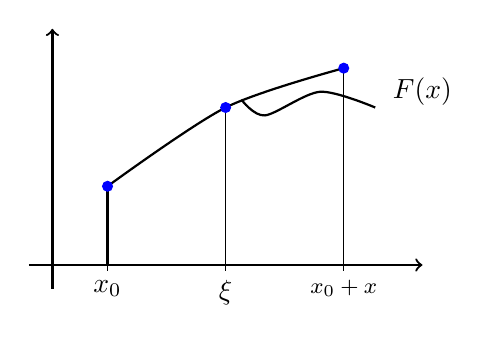
\begin{tikzpicture}
    			\draw[thick,->] (0,0) -- (5,0);
    			\draw[thick,->] (0.3,-0.3) -- (0.3,3);
    			\draw[thick] plot [smooth] coordinates {(1,1) (2.5,2) (4, 2.5)};
    			
    			\draw (1,2pt) -- (1,-2pt) node[anchor=north] {$x_0$};
    			\draw[thick,-] (1,0) -- (1,1);
    			\fill[blue,thick] (1,1) circle (2pt);
    			
    			\draw (2.5,2pt) -- (2.5,-2pt) node[anchor=north] {$\xi$};
    			\draw[thin,-] (2.5,0) -- (2.5,2);
    			\fill[blue,thick] (2.5,2) circle (2pt);
    			
    			\draw (4,2pt) -- (4,-2pt) node[anchor=north] {\footnotesize{$x_0+\varDelta x$}};
    			\draw[thin,-] (4,0) -- (4,2.5);
    			\fill[blue,thick] (4,2.5) circle (2pt);
    			
    			\draw (5,2.5) node[anchor=north] {$F(x)$};
    			
    			\draw[thick] plot [smooth] coordinates {(2.7,2.1) (3,1.9) (3.7, 2.2) (4.4,2)};
    		\end{tikzpicture}
    	\end{minipage}
    	\hspace{0.05\linewidth}
    	\begin{minipage}{0.65\linewidth}
    		Т.к. $\varDelta x$ <<мала>>, а $f$ непрерывна, то $f(\xi)\approx f(x_0)$
    		
    		~
    		
    		$P\{x_0\leq X\leq x_0+\varDelta x\}\approx f(x_0)\varDelta x$
    	\end{minipage}
    \end{minipage}
 	
 	\item $P\{X=x_0\}=\liml_{\varDelta x \rightarrow 0}P\{x_0\leq X\leq x_0+\varDelta x\}=\liml_{\varDelta x \rightarrow 0}f(\xi)\varDelta x\stackrel{\text{f непр. }\Rightarrow \text{ огр.}}{=}0$
 	
\end{enumerate}

\clearpage
